\section{Ideas preliminares}
Considere un experimento aleatorio y suponga que evoluciona o cambia de un estado a otro a lo largo del tiempo, y sea $X_t$ el estado del experimento al tiempo $t$ de tal forma que puede considerarse
que $X_t$ es una variable aleatoria para cada valor del índice $t$. Esta colección de variables aleatorias es la definición de proceso estocástico, y sirve como modelo para representar la evolución aleatoria de un sistema a lo largo del tiempo.\\
Las demostraciones de los resultados expuestos en este capítulo se pueden encontrar en\\\\
\begin{Def}
    Un proceso estocástico es una colección de variables aleatorias $\{X_t\}_{t\in T}$ definidas en algún espacio de probabilidad $(\Omega,\thinspace\mathscr{F})$, parametrizada por un conjunto $T$, llamado espacio parametral, en donde las variables aleatorias toman valores en un conjunto $S$ llamado espacio de estados.
    Por tanto, un proceso estocástico puede interpretarse como una sucesión de variables aleatorias cuyas características pueden variar a lo largo del tiempo.
\end{Def}
Se puede tener un espacio de estados discreto y un espacio de estados continuo.
En los casos más sencillos se toma como espacio parametral el conjunto
discreto $T= \{0, 1, 2,\ldots\}$ y estos números se interpretan como tiempos. En este caso se dice que el proceso es a tiempo discreto (también conocido como cadenas), y en general este tipo
de procesos se denotará por $\{X_n:\thinspace n= 0, 1, \ldots\}$ , o $\{X_n:\thinspace n= 0, 1, \ldots\}$ dependiendo de la complejidad de la notación de la variable aleatoria a utilizar.\\Así, para cada $n$, $X_n$ es es el valor del proceso o estado del sistema al tiempo $n$.
Se podría tomar como ejemplo a los cambios de que ocurren cada día, cada mes, cada año, etc.\\ En el caso del tiempo continuo, el espacio parametral se considera como el conjunto continuo $T=[0,+\infty)$ donde los cambios de estado se podrían realizar en cualquier instante.\\
A partir de ahora, seguiremos la convención de que si el subíndice de la variable aleatoria es $n$, entonces los tiempos son discretos; y si el subíndice es $t$, el tiempo se mide de manera continua\\
\begin{Ejm}
    Considere una máquina dentro de una fábrica. Los
    posibles estados para la máquina son que esté operando o que esté fuera de funcionamiento
    y la verificación de esta característica se realizará al principio de cada día de trabajo. Si
    hacemos corresponder el estado 'fuera de funcionamiento' con el valor 0 y el estado 'en operación' con el valor 1, nuestra colección de variables aleatoria está dada por 
    $$X_t=
    \label{ejm-procEstocástico}
    \begin{cases}
        0, & \mbox{Si la máquina está 'fuera de funcionamiento' en el tiempo $t$}\\
        1, & \mbox{Si la máquina está 'en operación' en el tiempo $t$}
    \end{cases}$$
    La figura (\ref{fig-procesoEstocástico-Ejemplo}) muestra una posible secuencia de cambios de estado a través del tiempo para esa máquina.
    \begin{center}
        \begin{figure}[htb]
            \begin{center}
             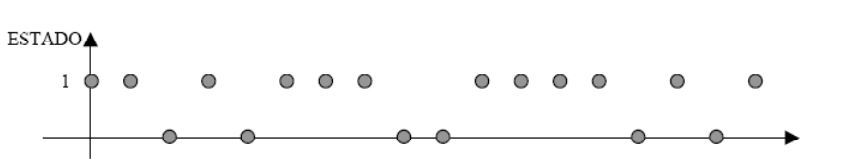
\includegraphics[width=14cm]{Cap2-ProcesosEstocásticos/img/ejem1.JPG}
                \vspace*{0.05in}
            \end{center}
            \caption{Estado que se encuentra la máquina al tiempo $t$ }
            \label{fig-procesoEstocástico-Ejemplo}
        \end{figure}
    \end{center}
    Según la gráfica, la máquina al tiempo $0$ y $1$ se encuentra en operación, por eso:
    $$X_0=1$$
    $$X_1=1$$
    Al tiempo $2$ la máquina cambia de estado y se encuentra fuera de funcionamiento. 
    $$X_2=0$$
    Y así sucesivamente vemos como la máquina va cambiando de estado constantemente a través del tiempo.
    $$X_3=1$$
    $$X_4=0$$
    $$\vdots$$
\end{Ejm}
\begin{Obs}
Para cualquier $t\in T$ se denota $P(X_t=i)$ o $P(X_t=i)$ para representar a la probabilidad que en el tiempo $t$ el ensayo está en el estado $i$. Esto es  $P(\omega\in\Omega,\thinspace X_t(\omega)=i).$
\end{Obs}
Un proceso estocástico, también llamado proceso aleatorio, puede considerarse como una función de dos variables
$$X:T\times\Omega\rightarrow S$$ a la cual a cada $(t,\thinspace\omega)$ se le asocia el valor o estado $X (t,\thinspace\omega) $.\\
Para cada valor de $t$ en $T$ , el mapeo $X_t$ o $X_t$ es una variable aleatoria, mientras que para cada $\omega$ en $\Omega$ fijo, la función $X(\cdot\thinspace,\thinspace\omega)$ es llamada una trayectoria o realización del proceso.\\En este trabajo estaremos interesados en el caso de procesos estocásticos con espacio de estados discreto, suele representarse de la siguiente
manera: $$(X_0=k_0,\thinspace\ldots,\thinspace X_n=k_n)$$
El principal interés del estudio a realizar en el caso discreto es el cálculo de probabilidades de ocupación de cada estado a partir de las probabilidades de cambio de estado. Si en el instante $n-1$ se encontraba en el estado $k_{n-1}$, ¿Con qué probabilidad se estará en el estado $k_n$ en
el estado siguiente $n$? Esta probabilidad de denotará como:
$$P(X_n = k_n\thinspace | \thinspace X_{n-1} = k_{n-1})$$
A este tipo de probabilidad condicionada se le denomina probabilidad de transición o de cambio de estado.\\Otra forma de denotarlo es $P(X_n = k_n\thinspace | \thinspace X_{n-1} := k_{n-1})=P_{i j}{(n-1,n)}$
\begin{Ejm}
    Del proceso estocástico expuesto en el ejemplo (\ref{ejm-procEstocástico}), \\$P_{0,1}(n-1,n)=P(X_n=1\thinspace|\thinspace X_{n-1}=0)$ denota la probabilidad de que en el tiempo $n$ la máquina esté 'en operación' , si previamente en el tiempo $n-1$ estaba 'fuera de funcionamiento'.\\
    $P_{1,0}(n-1,n)=P(X_{n-1}=0\thinspace|\thinspace X_n=1)$ denota la probabilidad de que en el tiempo $n$ la máquina esté 'fuera de funcionamiento', si previamente en el tiempo $n-1$ estaba 'en operación'.\\
    $P_{0,0}(n-1,n)=P(X_{n-1}=0\thinspace|\thinspace X_n=0)$ denota la probabilidad de que en el tiempo $n$ la máquina esté 'fuera de funcionamiento', si previamente en el tiempo $n-1$ también se encontraba 'fuera de funcionamiento'.
\end{Ejm}
Una propiedad interesante que se presentan en algunas cadenas es que los valores de sus probabilidades de transición no dependan del valor de $n$. Es decir, las probabilidades de cambiar de estado son las mismas en cualquier instante y no dependen del tiempo en que se encuentre el experimento, más bien lo relevante es el tiempo que transcurre en la transición. Esto es $$P_{i j}(0,n)=P_{i,j}(k,k+n),\quad \forall k\in\N$$ Por simplicidad se asumirá tal situación.\\
A este tipo de transiciones se le conoce como estacionarias y se denotan por simplicidad $P_{i,j}(n)$, en vez de $P_{i,j}(k,k+n)$ para cualquier $k\in T$, de esta manera se resalta que el tiempo transcurrido es $n$.\\
\begin{Obs}
    Sea $P_{i,j}(m,n)$ una probabilidad de transición estacionaria arbitraria. Por definición tenemos que $P_{i,j}(m,n)=P_{i,j}(n-m)$
\end{Obs}
\begin{Def}
    Sea  $\{X_t\}_{t\in T}$ un proceso estocástico con valores en el conjunto de estados $S=\{x_0,\thinspace x_1,\thinspace x_2 ,\ldots\}$ ( S puede ser finito o numerable ).
    Decimos que $\{X_t\}_{t\in T}$ es una cadena de Markov si cumple la siguiente propiedad conocida como la condición de Markov
    \begin{eqnarray}
    P(X_{n+1}=k_{n+1}\thinspace|\thinspace  X_{0}=k_0,\thinspace\ldots,\thinspace X_{n}=k_n)=P(X_{n+1}=k_{n+1}\thinspace|\thinspace X_{n}=k_n)
    \label{procesosEstocásticos-condMarkov}
    \end{eqnarray}
    Esto significa que la probabilidad de que el suceso $k_{n+1}$ ocurra en el tiempo $n+1$ (futuro) solo dependerá de la ocurrencia del evento $k_n$ en el tiempo $n$ (presente), mientras que la información de lo que ocurrió en los tiempos $0,\thinspace 1,\thinspace 2, \ldots,n-1$ (pasado) es irrelevante.
\end{Def}
\begin{Teo}
    La condición de Markov (\ref{procesosEstocásticos-condMarkov}) es equivalente a poder calcular la distribución conjunta de las variables $\{X_k\}_{k=1}^n$ de la siguiente forma:
    \begin{eqnarray}
    \label{procesosEstocásticos-condMarkovEquiv}
    P(X_0= k_0,\thinspace\ldots,X_{n+1}= k_{n+1}) =P(X_0=k_0)P(X_1=k_1|\thinspace X_0=k_0)\cdots P(X_{n+1}=k_{n+1}|\thinspace X_n=k_n)
    \end{eqnarray}
\end{Teo}
En general puede considerarse que una cadena de Markov inicia su evolución
partiendo de un estado $i$ cualquiera, o más generalmente considerando una
distribución de probabilidad inicial sobre el espacio de estados. Una distribución inicial para una cadena de Markov con espacio de estados $t= 0, 1,\thinspace 2,\thinspace,\ldots  $ es simplemente una distribución de probabilidad sobre este conjunto, es decir,
es una colección de números $p_0,\thinspace p_1,\thinspace p_2 ,\ldots$ que son no negativos y que suman uno. El número $p_i$ corresponde a la probabilidad de que la cadena inicie en el estado $i$, es decir $P(X_0= i)$\\ \\
\begin{Obs}
    En las cadenas de Markov en tiempo discreto, utilizábamos como índice un tiempo
    discreto $n=0, 1, 2,\ldots$ y se deducían numerosas propiedades.
    Las nociones de cadenas de Markov se puede extender a un tiempo continuo $t \geq 0$.
\end{Obs}
Consideremos un proceso a tiempo continuo $\{X_t\}_{t\leq 0}$ o que inicia en un estado $i_1$  al tiempo cero.
\begin{figure}
    \centering
    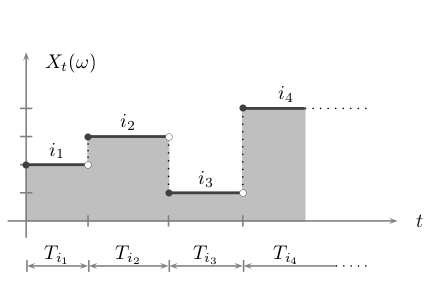
\includegraphics[width=10cm]{Cap2-ProcesosEstocásticos/img/procesos_continuos.png}
    \caption{Proceso estocástico a tiempo continuo}
    \label{fig-procEstocastContinuo}
\end{figure}
El proceso permanece en ese estado un tiempo aleatorio $T_{i 1}$, y
después salta a un nuevo estado $i_2$ distinto del anterior y así sucesivamente. Esta
sucesión de saltos se muestra gráficamente en la figura \ref{fig-procEstocastContinuo}
Los tiempos aleatorios $T$ son los tiempos
en los que el proceso permanece constante en alguno de sus estados, y se llaman tiempos de estancia.
Los momentos en donde el proceso tiene saltos son los tiempos $W_n=T_{i_1}+\cdots+T_{i_n}$ $n\in\N$.\\
Nuestro proceso estocástico $\{X_t\}_{t\leq 0}$ puede ser escrito como:
 $$X_t =
 \begin{cases}
    i_1, & \mbox{ Si $0\leq t <W_1$}\\
    i_2, & \mbox{ Si $0\leq t <W_1$}\\
    i_3, & \mbox{ Si $0\leq t <W_1$}\\
    \vdots
 \end{cases}$$
\begin{Def}
    Sea $\{X_t\}_{t\geq 0}$ un proceso estocástico sobre el conjunto de estados $S$, es una cadena de Markov de tiempo continuo si $S$ es numerable y para cualquier $0\leq t_1<t_2<\ldots<t_n<t_{n+1}$ se tiene  $$P\big(X_{t_n}=i_n\thinspace|\thinspace X_{t_1}=i_{t_1},\ldots ,\thinspace X_{t_{n-1}}=i_{t_{n-1}}\thinspace \big)=P\big(X_{t_n}=i_n\thinspace|\thinspace X_{t_{n-1}}=i_{t_{n-1}}\big)$$
\end{Def}
Observe que no estamos suponiendo que se conoce la historia del proceso en todo el pasado a tiempo continuo, sino únicamente en una colección arbitraria pero finita de tiempos pasados $t_1,t_2,t_3,\ldots,t_{n-1}$.\\
Supondremos nuevamente que estas probabilidades de transición son estacionarias en el tiempo, esto significa que para cada $s\leq 0$ y $t\leq 0$, la probabilidad $P(X_{t+s} =j \thinspace|\thinspace X_s= i)$ 
es idéntica a $P(X _{t} =j \thinspace|\thinspace X_0= i)$ , es decir, no hay dependencia del valor de $s$.
Esta probabilidad también se denota de manera breve mediante la expresión $P_{i j}(t)$, para $i$ y $j$ enteros no negativos.\\
\begin{Obs}
    En particular para $t= 0$, tanto para el caso continuo como discreto, se define la probabilidad de transición $P_{i j}(0)$ como la función delta de Kronecker, es decir,
    $$p_{i,j}(0)=\delta_{i j}=\begin{cases}
        1, & \mbox{Si $i=j$}\\
        0, & \mbox{Si $i\not= j$}
    \end{cases}$$
    Esto nos da a entender que, cuando el tiempo aún no transcurre, la probabilidad de que ocurra un cambio es nula, mientras que la probabilidad de que permanezca en el mismo estado es absoluta, es decir $1$.
\end{Obs}
Variando los índice $i$ y $j$, por ejemplo, sobre el conjunto de estados $t=\{ 1,\thinspace 2,\ldots, n\}$ , se
obtiene la matriz de probabilidades de transición de paso $t$, $t\geq 0$
$$P(t)=\left( \begin{array}{ccc}
p_{0 0}(t) & \cdots & p_{0 n}(t) \\ 
p_{1 0}(t) & \cdots & p_{1 n}(t)\\
\vdots & \ddots & \vdots \\
p_{n 0}(t) & \cdots & p_{n n}(t) 
\end{array}\right)\\$$
\begin{Ejm}
    En Perú existen $3$ operadores principales de telefonía móvil como lo son Movistar, Claro y Entel (estados).
    Los porcentajes actuales que tiene cada operador en el mercado actual son para Movistar $0.4$ para Claro $0.25$ y para Entel $0.35$. (estado inicial).
    Un usuario actualmente de Movistar tiene una probabilidad de permanecer en Movistar de $0.60$, de pasar a Claro $0.2$ y de pasarse a Entel de $0.2$.\\Si en la actualidad el usuario es cliente de Claro tiene una probabilidad de mantenerse en Claro del $0.5$, de que esta persona se cambie a Movistar  $0.3$ y que se pase a Entel de $0.2$.\\Si el usuario es cliente en la actualidad de Entel la probabilidad que permanezca en Entel es de $0.4$, de que se cambie a Movistar de $0.3$ y a Claro de $0.3$.\\
    Nuestra proceso estocástico estaría dado por $\{X_t\}_{t\leq 0}$ donde para dado tiempo $t\leq 0$, $\thinspace X_t(Movistar)=0$ ,$\thinspace X_t(Claro)=1$, $\thinspace X_t(Entel)=2$, partiendo de esta información podemos elaborar la matriz de transición.
   $$P(1)=\left( \begin{array}{ccc}
    P_{0 0}(1) & P_{0 1}(1) & P_{0 2}(1) \\
    P_{1 0}(1) & P_{1 1}(1) & P_{1 2}(1) \\
    P_{2 0}(1) & P_{2 1}(1) & P_{2 2}(1)  
    \end{array}\right)=
    \left( \begin{array}{ccc}
    0.60 & 0.2 & 0.2 \\ 
    0.3 & 0.5 & 0.2 \\
    0.3 & 0.3 & 0.4
    \end{array}\right)\\$$
    La suma de las probabilidades de cada estado en este caso operador deben ser iguales a $1$ y nuestro estado inicia en este caso sería $$P(X_0 = 0)= 0.4,\thinspace P(X_0 = 1)= 0.25 ,\thinspace P(X_0 = 2)= 0.35$$
    La probabilidad de que después de una temporada 
    Para descubrir cuál es la probabilidad de que una persona use Movistar en la época $0$ y luego use Claro en la época $1$. 
    $$P(X_1=1 , X_0=0) = P(X_0=0)P_{01}(1)= 0.40\cdot 0.20 =0.08$$
    Para descubrir cuál es la probabilidad de que una persona use Entel en la época $0$ y luego usar Movistar en la época $1$.
    $$P(X_1=0 , X_0=2) = P(X_0=2)P_{20}(1)=0.35\cdot 0.3 =0.105$$
    y si suponemos que nuestro proceso estocástico cumple la condición de Markov (\ref{procesosEstocásticos-condMarkov}) de pérdida de memoria, (no nos importa que operador haya usado mucho antes, solo nos interesa el operador usado previamente antes de la transición) entonces para calcular, por ejemplo la probabilidad de que una persona use Movistar en la época $0$ y luego use Claro en la época $1$ y finalmente Entel en la época $2$ usamos la condición equivalente (\ref{procesosEstocásticos-condMarkovEquiv}).
    $$P(X_2=2,\thinspace X_1=1,\thinspace X_0=0)=P(X_0=0)P_{01}(1)P_{12}(1)=0.4\cdot 0.2\cdot 0.2=0.016$$
    \end{Ejm}
\begin{comment}
    \begin{Teo}(Ecuación de Chapman-Kolmogorov)
        Para cualquier
        par de números enteros $m$ y $n$ tales que $0\leq m\leq n$, y para cualesquiera estados $i$ y $j$ se cumple
        \begin{eqnarray}
            p_{i,j}(m,n)=\sum_k p_{i,k}(m,u)P(u,t)
        \end{eqnarray}
    \end{Teo}
\end{comment}